\documentclass[10pt]{article}
\usepackage{a4wide}   % Mise en page une peu plus grande
\usepackage{hyperref} 
\usepackage{multicol} % pour pouvoir faire du multicols
\usepackage[french]{babel}  %
\usepackage{listings} % Pour faire de jolis listings
\usepackage{pifont}   % Pour les cmds dinglist et dingautolist
\usepackage{graphicx}
\usepackage[utf8]{inputenc} % Pour gérer les accents
\usepackage[T1]{fontenc}      % Gestion de la Cesure des mots accentues
\usepackage{dirtree}
\usepackage{float}

%qsfqsdfq
%%------------------------------------------------------------
%% Défintion de mes commandes
\newcommand{\G}[1]{\og #1 \fg}
\renewcommand{\baselinestretch}{1.3}
\setlength{\parskip}{1em}
\pagenumbering{gobble}

\usepackage[
backend=biber,
style=numeric,
sorting=ynt
]{biblatex}
 
\addbibresource{mybibliography.bib}





%%------------------------------------------------------------
%% Défintion du contenu du titre

\title{\begin{center}

\includegraphics[width=6cm]{pics/ENSIMAG-eps-converted-to.pdf}
\end{center} \vspace{1cm} Compte rendu TP 1}
\author{Auteur: Jan Bayer, Abderrazak Chaki, Alimata Djiré}

%%------------------------------------------------------------
%% Début du document
%%------------------------------------------------------------
\begin{document}
%% Implantation du titre
\maketitle
\newpage
%%------------------------------------------------------------
\tableofcontents
\newpage
\pagenumbering{arabic}
\section{Introduction}
Durant le cours de Génie logiciel, en programmation Java, nous avons eu pour projet la mise en place d’un programme qui nous permettra de visualiser et de modifier le contenu une base de données à travers l’interface Java Database Connectivity.
Le programme en langage Java devant être conforme au modèle MVC (modèle, vue, contrôleur) et utilisant la bibliothèque graphique Swing.
Dans ce compte rendu, nous allons définir rapidement les principes de la programmation orientée objet, puis on effectuera une analyse sur les différentes démarche que l’on aura suivi et on terminera par décrire les solutions adoptées pour l’implémentation du programme.
\section{Analyse}
La mise en \oe{}uvre de ce projet est basée sur les principes de la programation orientée objet. Dans cette section, on va introduire et expliquer les principes de ce paradigme et les spécificités en Java. 
\subsection{Programmation Orienté Objet}
Pour faciliter la simulation des objets réels, on a introduit la programmation orientée objet (POO). Ce paradigme permet de traduire des objets réels en objet informatique manipulable d’une manière plus logique et les regroupe dans une structure appelée classe. Une classe peut contenir plusieurs attributs et méthodes. Les attributs devront être initialisés et typés pour être correctement exploitable. Les méthodes quant à elles, peuvent utiliser ou non ces attributs, et si besoin créer ses variables locales.

La programmation orientée objet met en place ces trois principes de base:
\begin{itemize}
    \item \textbf{Encapsulation} : c’est le principe de regrouper des données et des méthodes au seins d’une structure.
    \item \textbf{Polymorphisme} : c’est le fait de pouvoir reprendre une structure existante et la modifier pour pouvoir l’adapter à notre besoin.
    \item \textbf{Héritage} : c’est la possibilité de créer une nouvelle classe à partir d’une classe déjà existante. Ainsi la classe fraîchement créée peut utiliser les attributs et les méthodes de sa  classe superieur.
\end{itemize}

\subsection{Java}
Java est un langage compilé (en bytecode) et interprété (par une JVM) qui est basé sur la programmation orientée objet. En effet, la particularité de Java est que tous ses composants sont des objets. Cela implique que les développeurs doivent créer une architecture la mieux adaptée à leur application.

Dans Java, on retrouve la notion du  packaging, c'est un concept qui lui est spécifique. Cette notion permet de regrouper des classes de façon organisée afin de faciliter la gestion des modules. Le fait de découper le programme en différents packages facilite son développement (en isolant les parties complexe), cela permet aussi de favoriser sa réutilisabilité c’est-à-dire l’aptitude à réutiliser tout le programme ou en partie pour alimenter une nouvelle architecture.

\begin{figure}[ht]
    \centering
    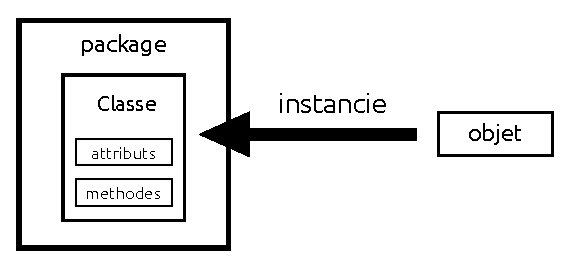
\includegraphics[width=10cm]{pics/classe.eps}
    \caption{Rélation entre les classes, objets et packages.}
    \label{fig:jvm}
\end{figure}

Les classes doivent être dans des fichiers portant le même nom qu’elles (le nom doit toujours commencer par une majuscule) et chaque classe peut être englobé dans un package (figure \ref{fig:jvm}). Chaque attribut, methodes et classes ont obligatoirement l'une des propriétés de visibilité suivantes:
\begin{itemize}
    \item \textit{privée} - visible uniquement dans la classe qui l’englobe
    \item \textit{protected} - visible aux classes descendante
    \item \textit{package-private} - visible aux classe dans le même package
    \item \textit{public} - visible aux seins d’une méthode)
\end{itemize}

Pour qu’une classe puisse réutiliser une autre d'un package different, il faut spécifier le chemin d'accès\footnote{On peut définir ce chemin en tant qu'un variable de l'environement ou l'option de script. } vers le répertoir racine de ce package.


\subsection{Analyse de projet}
Pour implémenter notre application nous utilisons des principes de la programmation orientée objets et des divers motifs de conception. Cette section décrit successivement des concepts utilisés dans notre projets dont MVC, des événements asynchrones et des principes d’interfaces graphiques.
 
\subsubsection{MVC}
La majorité des interfaces graphiques est basée sur le motif de Model-View-Controller (MVC), il devenait un standard pour l'implémentation des interfaces graphiques et des applications web. MVC nous permet de séparer les fonctions et de créer une architecture robuste pour gérer les données ainsi que l’interface graphique d’une manière indépendante. Le MVC est composé de trois éléments fondamentaux:
\begin{itemize}
    \item M - Model - est un composant qui manipule les données et souvent représente un accès au stockage de données (une base de donné, un disque dur \ldots)
    \item V - View - est un composant qui s’occupe des interactions avec un utilisateur et donc contient les éléments graphiques (fenêtre, panel, button \ldots)
    \item C - Controller - est un composant de la logique de l’application.
\end{itemize}

\subsubsection{Interfaces graphiques en Java}\label{interface_grap}
Les interfaces de base des interfaces graphiques sont déjà implementées dans la bibliothèque AWT qui se trouve dans le package \textit{java.awt} et donc fait partie de la version officielle de Java. C'est la bibliothèque AWT qui intéragit avec le système d'exploitation où l'interface graphique est gérées d'une façon asyncrhone\footnote{Les évènements arrivent de façon indepandante du programme}. La biblothèque AWT permet de signaler une arrivée d'un évenement comme le click de souris ou l'entrée du clavier. L'évenement est ensuite mis dans une liste d'attente pour les évenements graphiques et attend jusqu'à ce qu'un listeneur le récupere et procède à son traitement.
\newpage
\section{Implémentation}
Dans cette partie, nous allons expliquer les choix que nous avons adaptés pour la construction de notre programme. 
\subsection{Packaging}
On a composé la structure de l'application afin que chaque package répresente une fonnctionalité (voir la figure \ref{fig:packaging}). Le package \textit{controller} porte la logique de l'application et gère le comportement que vont adopter le modèle et la vue. Le package \textit{model} correspond au modèle de MVC et s'occupe de la gestion des entitées au sein du système grâce aux classes \textit{Model} et \textit{Person}. Il contient aussi la classe PersonDAO qui a pour but de créer une interface permettant la communication avec la base de donnée. Le package \textit{view} permet de faire l'affichage de l'interface graphique pour utilisateur. Il inclut la classe \textit{View} qui est l'executable de l'application.

\begin{figure}[ht]
    \centering
    \begin{minipage}{0.9\textwidth}
    \dirtree{%
    .1 com/ensimag/rie/mvcexo .
    .2 controller/.
    .3 ConnectToDb.
    .3 Controller.
    .2 model/.
    .3 dao/.
    .4 PersonDAO.
    .3 impl/.
    .4 PersonDAOImpl.
    .3 Model.
    .3 Person.
    .2 view/.
    .3 View.
    .3 AddPersonButton.
    .3 DeletePersonButton.
    .3 PersonPanel.
    .2 services/impl/.
    .3 PersonService.
    .2 exceptions/.
    .3 Service Exception. 
    }
    \end{minipage}
    \caption{Arboresance des packages}
    \label{fig:packaging}
\end{figure}

Le package \textit{exceptions} est composé des exceptions qui peuvent être jetées par l'application. Le package \textit{service} offre une couche intermediaire entre le controleur et le modèle.

\subsection{Connexion à la base de donnée}
Le langage Java dispose d'une interface qui facilite la connexion à la base de donnée, notamment les BDD relationnelles. Cette interface s'appelle \textit{Java Database Connectivity} et se trouve dans le package \textit{java.sql}. Elle définit la manière de la programmation des pilotes pour les divers BDD et en même temps elle met en jeu l'interface de la connexion pour les applications (figure \ref{fig:jdbc}). JDBC ne fournit que les interfaces sans implementation, pour cette raison on a dû  télécharger les pilots JDBC Oracle (en forme d'une archive JAR). On a inclut cette archive dans notre Classpath et on a indiqué à JDBC le fourniseur des pilotes à travers l'URL (qui est spécifique pour chaque implementation de JDBC).

\begin{figure}[ht]
    \centering
    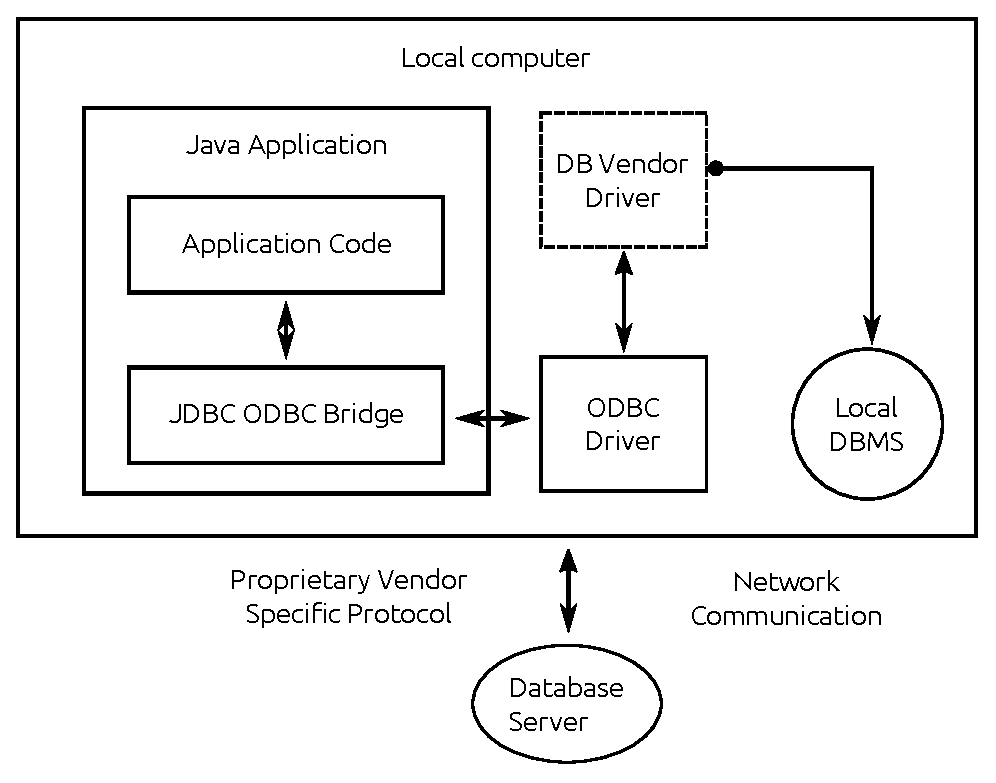
\includegraphics[width=10cm]{pics/jdbc.eps}
    \caption{Rélation entre les classes, objets et packages. \cite{TutorialsPoint} La figure répresente la communication entre l'application Java, JDBC et le serveur de la BDD. Le code d'applicatione échange avec le pilote ODBC qui crée une copie local du schéma présent dans le serveur (Local DBMS). Les changements sont mergé après la validation (\textit{COMMIT} en SQL).}
    \label{fig:jdbc}
\end{figure}

\subsection{Action Listener}
Le principe décrit dans la section \ref{interface_grap} est basé sur les arrivée des évènements asynchronnes auxquels on assigne une classe qui gère leurs traitement : Action Listener. Cette classe doit impérativement implementer l'interface \textit{ActionListener} qui est disponible dans la bibliothèque AWT. Dans notre application, ce composant est présent dans la classe \textit{Controller}, il définit les actions pour le modèle et la vue. 

\subsection{Swing et Layouts}
ATW est une bibliothèque qui accède directement à l'interafce graphique native du système d'exploitation ce qui peut empecher les applications d'être portable. Pour pallier à ce problème, Java a mis en place une autre bibliothèque graphique qui est partialement basée sur AWT mais qui permet de porter les applications entre les differents plateformes. 

Notre application crée la fênetre en utilisant la classe \textit{JFrame} et utilse les layouts suivants:
\begin{itemize}
    \item \textbf{BorderLayout} - la mise en page des élément basé sur l'orientation (nord, sud, est, ouest et centre)
    \item \textbf{BoxLayout} - la mise en page qui a le même comportement qu'une cascade et on l'utilise pour afficher les buttons pour supprimer de chaque perssonne. 
    \item \textbf{FlowLayout} - la mise en page qui empile les éléments en ligne.
\end{itemize}

\section{Problèmes rencontrés}
\begin{enumerate}
    \item \textbf{URL de la BDD} Le premier problème était de trouver le bon URL pour pouvoir accéder à la base de donner de l'ENSIMAG. Comme le système de l'URL est propre à Oracle, il était difficile de comprendre son sense et choisir le bon.
    \item \textbf{JDBC par Oracle} Comme les pilotes d'Oracle ne sont pas instalés par defaut, il fallait les télécharger sur leur site-web en forme d'une archive JAR. On devait l'inclure dans notre Classpath.
    \item \textbf{Layouts} AWT et Swing offrent beaucoup de possibilités d'implementation de mise en page en utilisant les \textit{LayoutManager} dont principes ne sont pas évident et donc il fallait essayer presque tous.
\end{enumerate}
\section{Conclusion}
Ce projet nous a permis de mettre en pratique les notions apprises en cours, de pouvoir les développer et de comprendre ou découvrire de nouvelles solutions lors qu'on a été confrontés à des problèmes. Nous avons aprécier l'apprentissage à travers la documentation officielle Java. 

Le code source est disponible sur ce repository Git: https://github.com/bayerhonza/mvcexo  
\newpage
\printbibliography
\end{document}
